\chapter{Программа}\label{ch:program}

Во время работы были написаны программа на языке Python, реализующая расчёты по методу <<крест-колокол>>.
Она состоит из следующих модулей
\begin{enumerate}
    \item config - чтение конфигурационных файлов для задач
    \item mesher - генерации расчётной сетки для системы
    \item solver - расчёта деформаций и разрыва тканного композита
    \item writer - запись результатов в формат .vtu (VTK Unstructured Grid)
\end{enumerate}
Далее подробно рассмотрим каждый модуль.

\section{Config}\label{sec:prog-config}
Config - модуль, отвечающий за чтение списка задач для программы.

Конфиг представляет собой список задач (tasks) и директорию, для записи результатов (out\_dir).
Каждый task имеет вид:
\begin{minted}{yaml}
name: simple # название таска, результат будет иметь вид: ${name}.vtu
mesh:
    resolution: 100 # Разрешение нитей, точек/см
    diameter: 0.5 # толщина нити, см
    width: 20 # Ширина куска = длина ниток утка
    weft_density: 1 # Плотность ниток утка, нитей / см
    length: 50 # Длина куска = длина ниток основы
    warp_density: 0.5 # Плотность ниток основы, нитей / см
solver:
    n_steps: 250 # Число шагов
    step: 0.1 # размер шага
    pulse:
        radius: 5 # Радиус нагрузки
        amplitude: 1 # Амплитуда нагрузки
        center: # Точка нагрузки
            x: 50
            y: 50
            z: 0
\end{minted}

Конфиг поддерживает шаблоны jinja2 для быстрой генерации параметризованных задач.

Пример полного конфига
\begin{minted}{yaml}
---
out_dir: out

tasks:
  - name: simple
    mesh:
      resolution: 1
      diameter: 0.001
      width: 100
      weft_density: 1
      length: 100
      warp_density: 1
    solver:
      step: 0.1
      n_steps: 250
      pulse:
        radius: 5
        amplitude: 1
        center:
          x: 50
          y: 50
          z: 0
  
  - name: "step-{{ step }}"
    mesh:
      resolution: 1
      diameter: 0.001
      width: 100
      weft_density: 1
      length: 100
      warp_density: 1
    solver:
      step: !!float "{{ step }}"
      n_steps: !!int "{{ (25/step)|round|int }}"
      pulse:
        radius: 5
        amplitude: 1
        center:
          x: 50
          y: 50
          z: 0
  
\end{minted}

\section{Mesher}\label{sec:prog-mesher}
Mesher - модуль отвечающий за генерацию сетки из тонких нитей.
Принимает на вход данные из секции mesh в задаче из \ref{sec:prog-config}.

Для оптимизации вычислений используется следующий алгоритм.

Все нити в слое делятся на два типа - основа и ут\'{о}к. Основа - прямые нити, вокруг которых оплетаются нити утка.

Далее для основы генерится одна нить и параллельным переносом создаётся группа нитей.

Для утка так же генерится одна нить, но сложнее: сперва описание нити разбивается на повторяющиеся части, как в
\picref{fig:weft-fiber}

\begin{figure}[H]
    \centering
    \caption{Часть утка крупным планом}
    \label{fig:weft-fiber}
    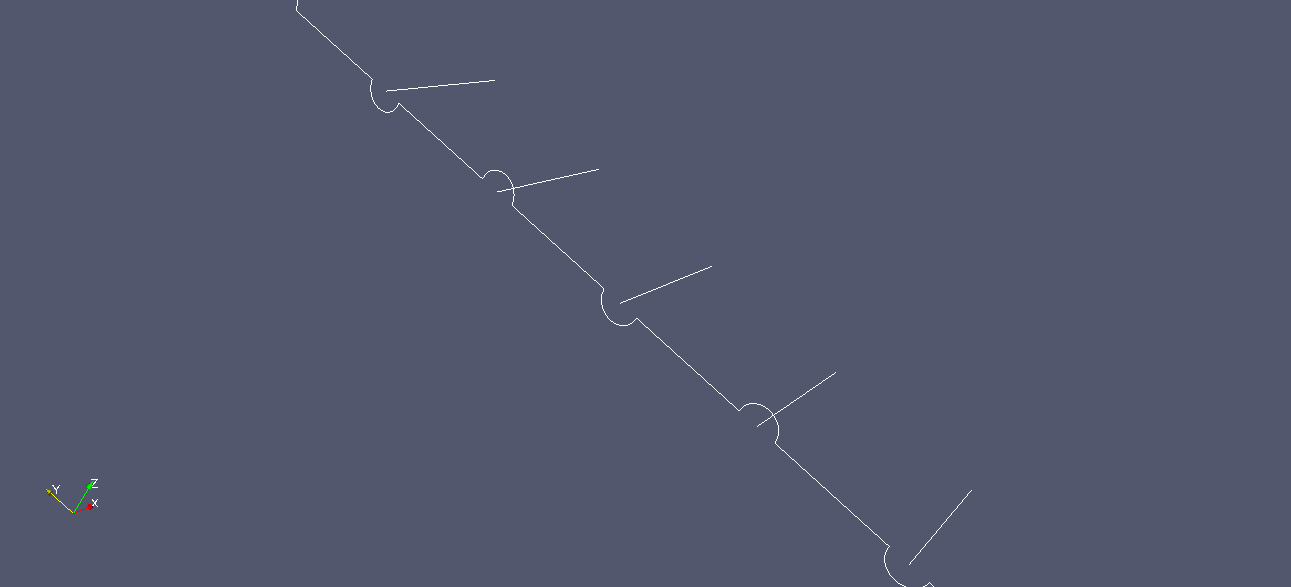
\includegraphics[width=1.0\textwidth]{img/weft_fiber.png}
\end{figure}

Затем она повторяется до полной нити.

В конце все нити сводятся до состояния как на \picref{fig:scheme}
\begin{figure}[H]
    \centering
    \caption{Вид на сетку сверху}
    \label{fig:scheme}
    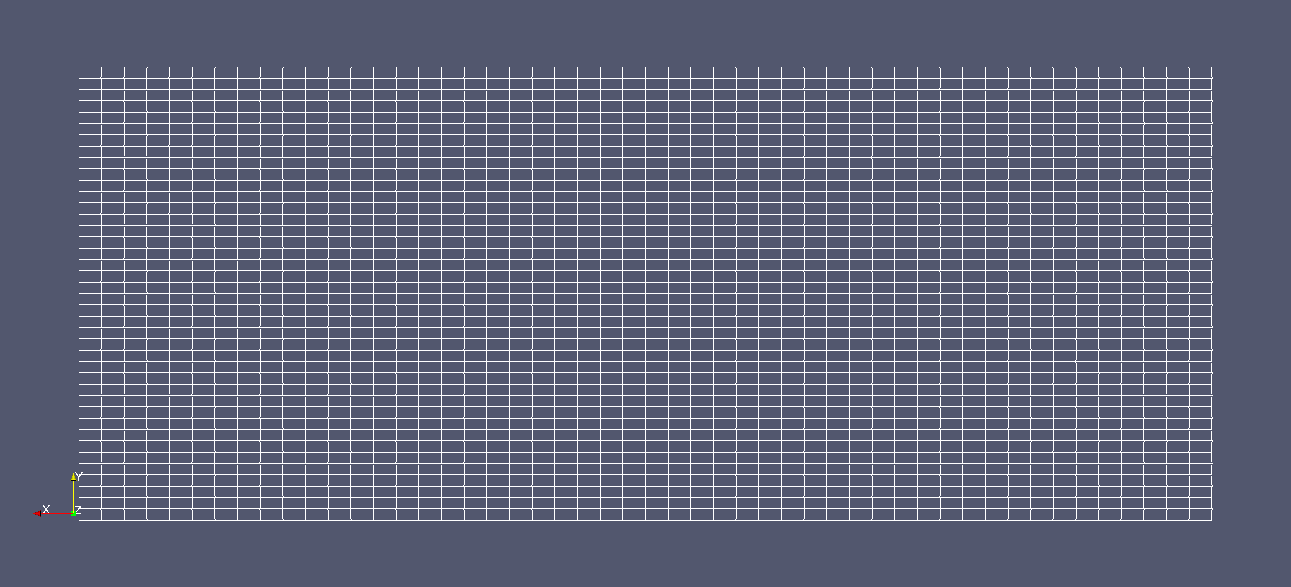
\includegraphics[width=1.0\textwidth]{img/scheme.png}
\end{figure}

\section{Solver}\label{sec:prog-solver}
Solver - модуль, считающий деформации в слое ткани.

Принимает на вход параметры, описанные в секции solver из \ref{sec:prog-config}.

\section{Writer}\label{sec:prog-writer}
Writer - модуль, записывающий результаты в формате, подходящем для визуализации с помощью Paraview.
